\chapter{Diseño e Implementación} % Main chapter title

\label{Chapter3} % Change X to a consecutive number; for referencing this chapter elsewhere, use \ref{ChapterX}
\definecolor{mygreen}{rgb}{0,0.6,0}
\definecolor{mygray}{rgb}{0.5,0.5,0.5}
\definecolor{mymauve}{rgb}{0.58,0,0.82}

\lstset{ %
  backgroundcolor=\color{white},   % choose the background color; you must add \usepackage{color} or \usepackage{xcolor}
  basicstyle=\footnotesize,        % the size of the fonts that are used for the code
  breakatwhitespace=false,         % sets if automatic breaks should only happen at whitespace
  breaklines=true,                 % sets automatic line breaking
  captionpos=b,                    % sets the caption-position to bottom
  commentstyle=\color{mygreen},    % comment style
  deletekeywords={...},            % if you want to delete keywords from the given language
  %escapeinside={\%*}{*)},          % if you want to add LaTeX within your code
  %extendedchars=true,              % lets you use non-ASCII characters; for 8-bits encodings only, does not work with UTF-8
  %frame=single,	                   % adds a frame around the code
  keepspaces=true,                 % keeps spaces in text, useful for keeping indentation of code (possibly needs columns=flexible)
  keywordstyle=\color{blue},       % keyword style
  language=[ANSI]C,					% the language of the code
  %otherkeywords={*,...},           % if you want to add more keywords to the set
  numbers=left,                    % where to put the line-numbers; possible values are (none, left, right)
  numbersep=5pt,                   % how far the line-numbers are from the code
  numberstyle=\tiny\color{mygray}, % the style that is used for the line-numbers
  rulecolor=\color{black},         % if not set, the frame-color may be changed on line-breaks within not-black text (e.g. comments (green here))
  showspaces=false,                % show spaces everywhere adding particular underscores; it overrides 'showstringspaces'
  showstringspaces=false,          % underline spaces within strings only
  showtabs=false,                  % show tabs within strings adding particular underscores
  stepnumber=1,                    % the step between two line-numbers. If it's 1, each line will be numbered
  stringstyle=\color{mymauve},     % string literal style
  tabsize=2,	                   % sets default tabsize to 2 spaces
  title=\lstname,                   % show the filename of files included with \lstinputlisting; also try caption instead of title
  morecomment=[s]{/*}{*/}%
}

% -------------------------------------

En este capítulo se muestra todo el proceso de desarrollo del dispositivo, tanto el firmware como hardware, a partir del modelo de desarrollo aplicado..
% --------------------------------------


\section{Implementación del sistema}

\subsection{Resumen del sistema}

El equipo digitaliza señales analogicas provenientes de dos sensores de presión intrarterial del tipo strain-gauge y almacena las señales por períodos prolongados de alrededor de 24 hs. Estas señales adquiridas se guardan en una memoria de tipo flash (memoria SD), y pueden descargarse a una PC a través de una interfaz USB. Desde la PC se accede a los archivos guardados como un medio de almacenamiento masivo, y se pueden visualizar en cualquier software que permita procesar un archivo de tipo ".csv".

Previo a cada experiencia, el operador configura el equipo desde una terminal Bluetooth, como una tablet o una PC, a través de un protocolo de comunicación muy sencillo que se desarrolló para este dispositivo. A través de esta interfaz se configuran parámetros como la frecuencia de muestreo, la cantidad de canales a usar, ganancia del amplificador programable, seteo de hora y fecha, y finalmente se da inicio a la medición. 

El equipo consiste en un sistema embebido portátil basado en un microcontrolador ARM de 32 bits, Cortex M3: LPC1769, un conversor analógico digital de alta resolución (ADS1292), módulos de comunicación (serie, BLE, USB), almacenamiento masivo (SD) y módulo de regulación de energía y carga de batería. Puede verse un diagrama en bloques en la Figura \ref{fig:diag_bloques} . Para este proyecto se utilizaron en forma intensiva la gran mayoría de los contenidos y herramientas vistas durante el Carrera de Especialización en Sistemas Embebidos (CESE). Se utilizaron técnicas de Gestión de Proyectos, documentación manual y automática del trabajo, sistema de versionado de software y hardware. En cuanto a lo técnico se emplearon conocimientos específicos sobre arquitectura del microcontrolador, modelos de programación, sistema operativo de tiempo real freeRTOS, protocolos de comunicación (BLE, SPI, USB, y de alto nivel), testing unitarios, etc.


\begin{figure}[!htbp]
	\centering
	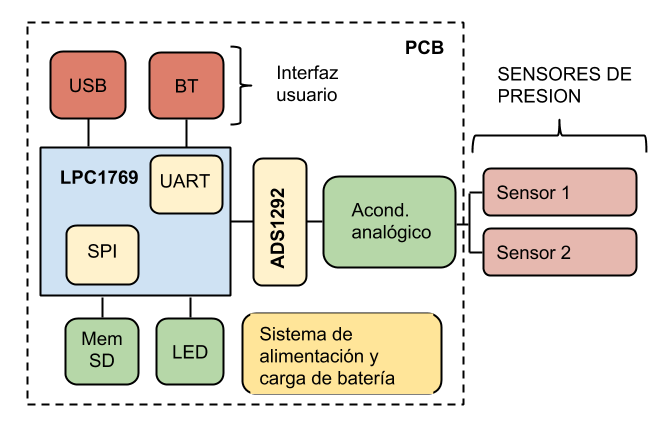
\includegraphics[width=\textwidth]{./Figures/diag_bloques.png}
	\caption{Diagrama en bloques del equipo.}
	\label{fig:diag_bloques}
\end{figure}

\subsection{Modelo de desarrollo del firmware}


El proceso elegido para el desarrollo del firmware es el modelo en V. Se trata de un modelo descripto en términos de un proceso de construcción descendente ("Software Development Life Cycle", SDLC) y un proceso de verificación y validación ascendente ("Software Test Life Cycle", STLC) \citep{fowler2015}. El punto que une estos dos procesos es la implementación del código. 
Durante el proceso descendente se descomponen y clarifican las necesidades del cliente, dando lugar a los requisitos específicos, diseño de la arquitectura en términos generales y diseño detallado de cada uno de los bloques de código. Luego, cada uno de estos niveles de la fase de construcción se asocia con un nivel de la fase de pruebas, dando lugar a las pruebas unitarias, pruebas de integración y pruebas de sistema.

\begin{figure}[!htbp]
	\centering
	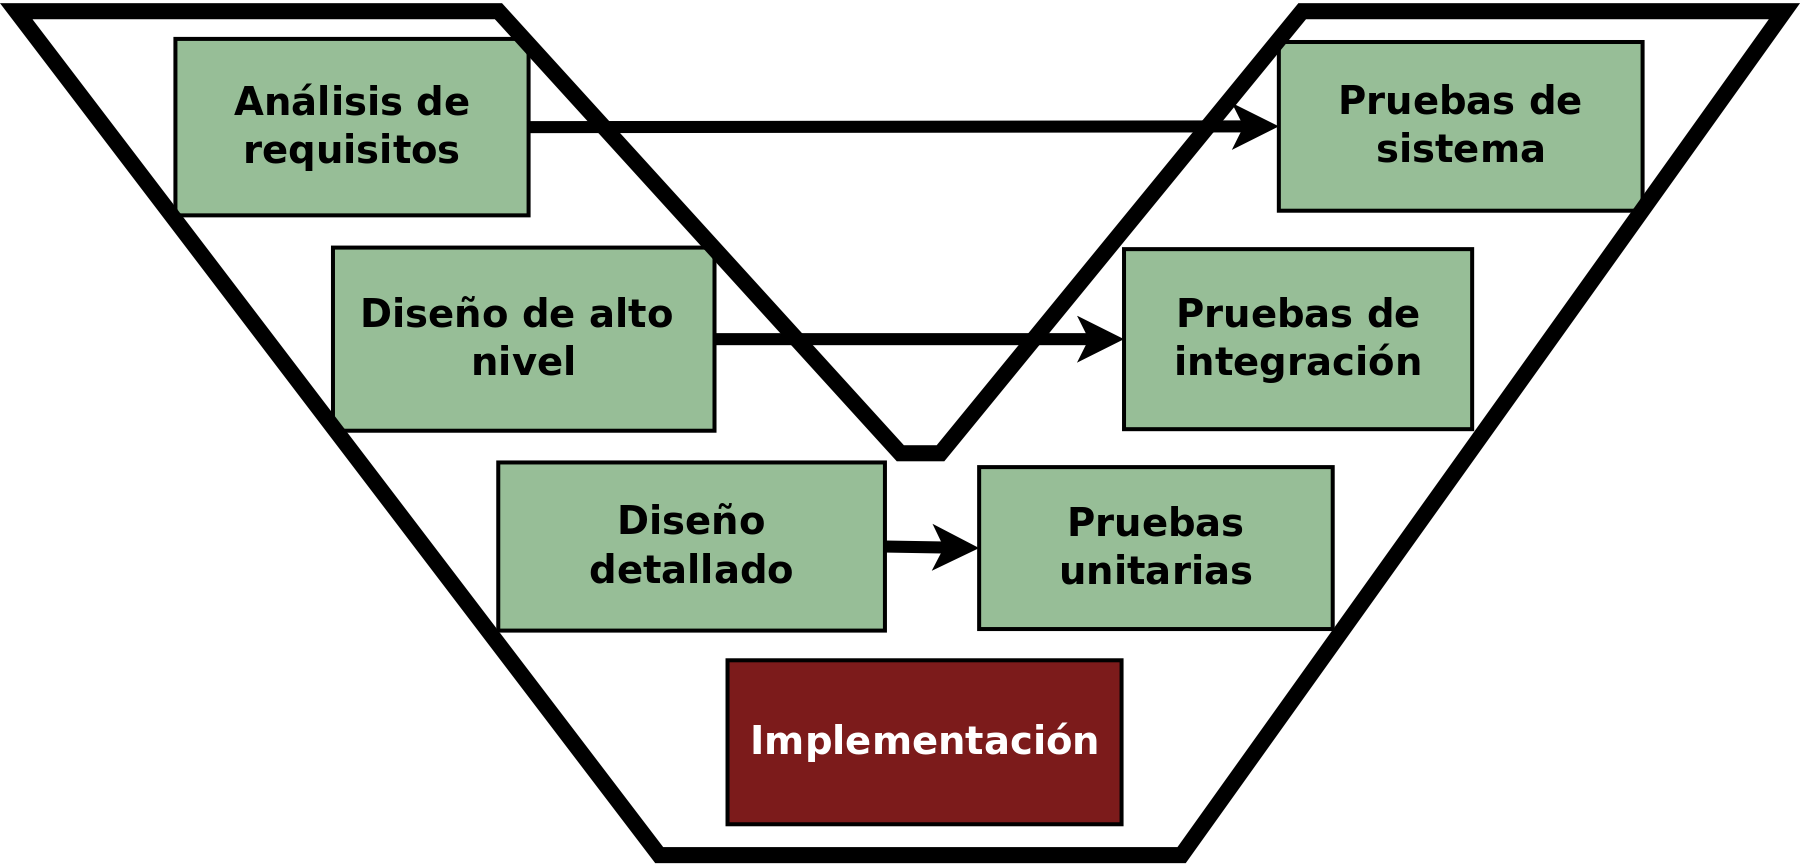
\includegraphics[width=\textwidth]{./Figures/modeloV.png}
	\caption{Modelo de desarrollo y validación en V}
	\label{fig:modeloV}
\end{figure}

A continuación se pone en relieve cada una de estas instancias del proceso de desarrollo.

\subsection{Analisis de los requerimientos}

A partir de un análisis de los requerimientos explicitados en el capítulo anterior se puede determinar que los Requerimientos 1 y 2 están estrictamente asociados al hardware. Se puede ligar alguno de estos requerimientos al firmware, como por ejemplo el R1.1 ya que el firmware es el responsable de la entrada a modos de bajo consumo o la administración de energía dentro del microcontrolador. Sin embargo, la mayor carga de responsabilidad de cumplimiento de estos requerimientos están volcados sobre el hardware. Los requerimientos 3 y 4 están muy ligados al desarrollo del firmware del equipo. Solamente el requerimiento 4.2 está relacionado al tamaño de la memoria utilizada que es una cuestión de hardware.
Por otro lado, la lista de requerimientos del capítulo anterior no es exhaustiva y da por supuesto las funcionalidades básicas del equipo. Se elaboraron una serie de requerimientos más específicos sobre el funcionamiento detallado de la operación del usuario y los parámetros que es posible configurar. 


\begin{enumerate}

	\setcounter{enumi}{4}

	\item \textbf{Requerimientos estructurales:} 
	\begin{enumerate}[label*=\arabic*.]
		\item El equipo debe poder adquirir señales analógicas de hasta dos canales de entrada.
		\item El desfasaje entre las señales adquiridas debe ser nulo.
		\item El equipo debe inicializar solamente los periféricos que se utilicen en el momento adecuado para ahorrar energía. 
	\end{enumerate}
	
	\item \textbf{Requerimientos operativos:}
	\begin{enumerate}[label*=\arabic*.]
		\item Al estar inactivo, el equipo debe entrar en modo configuración para poder ponerse en hora y mantenerla mientras tenga batería.
		\item Al estar en configuración, se debe poder chequear el correcto funcionamiento del hardware (SD, conversor AD, etc).
		\item Si el equipo esta inactivo, al enviar un comando desde la terminal, se comienza a adquirir y enviar vía bluetooth (esta señal puede estar decimada y con menor resolución) con la configuración previamente seleccionada.
		\item Si el equipo está adquiriendo y enviando vía bluetooth, se puede enviar una orden para que el equipo finalice y vuelva al modo inactivo.
		\item Si el equipo está adquiriendo y enviando vía bluetooth, se puede enviar una orden para que el equipo comience a almacenar en la memoria SD.
		\item Si se esta adquiriendo, enviando señal vía bluetooth y almacenando en la SD, se debe poder enviar una orden para que el equipo deje de hacerlo y vuelva al modo inactivo.
		\item Si se esta adquiriendo, almacenando y enviando por Bluetooth, se debe poder enviar una orden para que el equipo deje de enviar la señal por Bluetooth y continúe la experiencia en forma silenciosa.
		\item Si el equipo está adquiriendo y almacenando en forma silenciosa, se debe poder enviar un comando para que vuelva a enviar la señal por Bluetooth sin interrumpir ni alterar la adquisición y almacenamiento.
		\item Si el equipo está adquiriendo, enviando señal via Bluetooth y almacenando, se puede enviar un comando para que el equipo deje almacenar.
		\item Si el equipo esta inactivo, se puede requerir el envío de una señal patrón para chequeo del canal de comunicación.
		\item Si el equipo esta enviando la señal patrón para chequeo de canal de comunicación, se puede enviar un comando para que el equipo vuelva a modo inactivo.
		\item Se debe almacenar por cada registro la hora, los canales activados y el nivel de batería.
		\item Cada vez que se comienza un nuevo almacenamiento, se genera un archivo nuevo con nombre auto numerado.
		\item Cada vez que comienza o finaliza un almacenamiento, se registra en un archivo que debe contener el nombre del archivo y la fecha y hora de inicio y fin de todas las experiencias.
		\item Cada uno de estos modos debe estar señalizado por uno o mas leds para comprobar visualmente el funcionamiento.
	\end{enumerate}
	
	\item \textbf{Requerimientos de configuración}
	
	\begin{enumerate} [label*=\arabic*.]
		\item El equipo debe tener una configuración por default y la posibilidad de modificarla mientras no se esta adquiriendo.
		\item El equipo debe poder volver a la configuración de fábrica.
		\item El equipo debe guardar la última configuración y utilizarla.
		\item Se debe poder elegir la frecuencia de muestreo dentro de algunas opciones.
		\item Se debe poder elegir si activar uno o los dos canales.
		\item Se debe poder elegir la ganancia del amplificador.
		\item El equipo se debe poder calibrar con dos puntos de presión conocidos.		
	\end{enumerate}


\end{enumerate}


De toda la lista completa de requerimientos surgen los casos de uso con operaciones básicas del usuario. A continuación se muestran los diferentes casos de uso que se desprenden de los requerimientos:

	\textbf{Caso de uso CU0001:}

	\begin{enumerate} 
		\item Nombre: CU0001
		\begin{enumerate} [label*=\arabic*.]
			\item Descripción: Autonomía
			\item Actor Principal: Usuario
			\item Disparador: Encendido del equipo		
		\end{enumerate}
		\item Flujo de eventos
		\begin{enumerate} [label*=\arabic*.]
			\item Flujo básico: el usuario enciende el equipo, realiza la configuración y comienza la experiencia. Luego de 24 hs finaliza la experiencia desde una terminal.
			\item Flujo alternativo: Si la batería no tiene carga total, es responsabilidad del usuario. Según la configuración se puede calcular autonomía aproximada.
		\end{enumerate}

		\item Requerimientos especiales: conexión Bluetooth
		\item Pre-condiciones: cargar la batería al 100\% antes de comenzar a usar el equipo.
		\item Post-Condiciones: Finalizar correctamente la experiencia.				
	\end{enumerate}

	\textbf{Caso de uso CU0002:}

	\begin{enumerate} 
		\item Nombre: CU0002
		\begin{enumerate} [label*=\arabic*.]
			\item Descripción: Configuración
			\item Actor Principal: Usuario
			\item Disparador: Ingreso a configuración desde la terminal
		\end{enumerate}
		\item Flujo de eventos
		\begin{enumerate} [label*=\arabic*.]
			\item Flujo básico: el usuario desde la terminal ingresa al modo configuración, modifica los parámetros que necesita o calibra un canal, y vuelve a salir del modo configuración.
			\item Flujo alternativo:
			\begin{itemize}
				\item Si el equipo no está sincronizado, indica error y da la oportunidad de reiniciar. 
				\item Si no se puede abrir la última configuración, debe abrir la configuración de fábrica y mostrar error.
				\item La nueva configuración elegida se guarda y se comprueba al comenzar la experiencia. Hasta ese momento no se comprueba si es correcta.
				\item Si se comprueba algún error de hardware, se debe enviar un mensaje de reparación.						
			\end{itemize}				
		\end{enumerate}

		\item Requerimientos especiales: conexión Bluetooth
		\item Pre-condiciones: equipo en modo inactivo
		\item Post-Condiciones: salir correctamente del modo configuración.
	\end{enumerate}



	\textbf{Caso de uso CU0003:}

	\begin{enumerate} 
		\item Nombre: CU0003
		\begin{enumerate} [label*=\arabic*.]
			\item Descripción: Experiencia
			\item Actor Principal: Usuario
			\item Disparador: Ingreso a experiencia desde la terminal
		\end{enumerate}
		\item Flujo de eventos
		\begin{enumerate} [label*=\arabic*.]
			\item Flujo básico: el usuario desde la terminal ingresa al modo de adquisición y visualización, comprueba el correcto funcionamiento de los sensores habilitados observando la señal adquirida. Luego ingresa al modo almacenamiento y comprueba que no haya error en el almacenamiento de datos. Luego selecciona dejar de enviar para que la experiencia continúe en modo silencioso. Al finalizar la experiencia, el usuario envía la orden para terminar la adquisición. El usuario luego comprueba que la adquisición fue completa.
			\item Flujo alternativo:
			\begin{itemize}
				\item Si los sensores no muestran una señal adecuada, se debe salir de la adquisición y chequear conectores.
				\item Si los sensores no muestran ninguna señal, se debe comprobar el canal.
				\item Si hay error al comenzar a almacenar, se detiene la adquisición para comprobar el funcionamiento de la tarjeta SD.
				\item Si se necesita ver las señales por una eventual desconexión, se puede conectar mediante bluetooth para visualizar las señales y luego salir. 
				\item Si no se puede volver a conectar con la terminal, se debe acceder físicamente a conectar el equipo a una PC.
				\item Si la batería esta en un nivel crítico, el equipo debe guardar el archivo y finalizar la experiencia. El usuario se notifica de esto al intentar conectarse.					
			\end{itemize}				
		\end{enumerate}

		\item Requerimientos especiales: conexión Bluetooth
		\item Pre-condiciones: equipo en modo inactivo
		\item Post-Condiciones: salir correctamente de la experiencia.
	\end{enumerate}


	\textbf{Caso de uso CU0004:}

	\begin{enumerate} 
		\item Nombre: CU0004
		\begin{enumerate} [label*=\arabic*.]
			\item Descripción: Experiencia
			\item Actor Principal: Usuario
			\item Disparador: Ingreso a experiencia desde la terminal
		\end{enumerate}
		\item Flujo de eventos
		\begin{enumerate} [label*=\arabic*.]
			\item Flujo básico: el usuario desde la terminal ingresa al modo de adquisición y visualización, comprueba el correcto funcionamiento de los sensores habilitados observando la señal adquirida. Luego ingresa al modo almacenamiento y comprueba que no haya error en el almacenamiento de datos. Luego selecciona dejar de enviar para que la experiencia continúe en modo silencioso. Al finalizar la experiencia, el usuario envía la orden para terminar la adquisición. El usuario luego comprueba que la adquisición fue completa.
			\item Flujo alternativo:
			\begin{itemize}
				\item Si los sensores no muestran una señal adecuada, se debe salir de la adquisición y chequear conectores.
				\item Si los sensores no muestran ninguna señal, se debe comprobar el canal.
				\item Si hay error al comenzar a almacenar, se detiene la adquisición para comprobar el funcionamiento de la tarjeta SD.
				\item Si se necesita ver las señales por una eventual desconexión, se puede conectar mediante bluetooth para visualizar las señales y luego salir. 
				\item Si no se puede volver a conectar con la terminal, se debe acceder físicamente a conectar el equipo a una PC.
				\item Si la batería esta en un nivel crítico, el equipo debe guardar el archivo y finalizar la experiencia. El usuario se notifica de esto al intentar conectarse.					
			\end{itemize}				
		\end{enumerate}

		\item Requerimientos especiales: conexión Bluetooth
		\item Pre-condiciones: equipo en modo inactivo
		\item Post-Condiciones: salir correctamente de la experiencia.
	\end{enumerate}

\textbf{Caso de uso CU0005:}

	\begin{enumerate} 
		\item Nombre: CU0005
		\begin{enumerate} [label*=\arabic*.]
			\item Descripción: Descarga de datos y carga de batería.
			\item Actor Principal: Usuario
			\item Disparador: Conectar el equipo por USB a PC
		\end{enumerate}
		\item Flujo de eventos
		\begin{enumerate} [label*=\arabic*.]
			\item Flujo básico: el usuario conecta el equipo a la PC y comprueba que se reconozca como un medio de almacenamiento masivo. Luego descarga los archivos que sean necesarios y deja el equipo conectado mientras necesite cargar la batería. Finalmente, luego de finalizadas todas las transferencias de datos, desconecta el equipo del USB.
			\item Flujo alternativo:
			\begin{itemize}
				\item Si la PC no reconoce al equipo como medio de almacenamiento masivo, se debe comprobar la tarjeta SD.
				\item Si el equipo no carga la batería, se debe hacer una revisión técnica del equipo y de las baterías.			
			\end{itemize}				
		\end{enumerate}

		\item Requerimientos especiales: conexión USB
		\item Pre-condiciones: equipo en modo inactivo
		\item Post-Condiciones: desconectar el USB cuando no haya ninguna transferencia activa y cuando haya terminado de cargar la batería. El nivel de batería se puede comprobar desde la terminal entrando al modo configuración.
	\end{enumerate}
	
A partir de los requerimientos y casos de usos armamos la matriz de trazabilidad, que consiste en una tabla de doble entrada que asocia cada requerimiento con uno o más casos de uso.

\textbf{Matriz de Trazabilidad}

%Please add the following required packages to your document preamble:
% \usepackage{booktabs}
% \usepackage[table,xcdraw]{xcolor}
% If you use beamer only pass "xcolor=table" option, i.e. \documentclass[xcolor=table]{beamer}
% \usepackage{longtable}
% Note: It may be necessary to compile the document several times to get a multi-page table to line up properly
\begin{longtable}[c]{@{}lllllll@{}}

\caption{Matriz de Trazabilidad}
\toprule
% \rowcolor[HTML]{DAE8FC} 
\textbf{REQ/CU} & \textbf{CU0001} & \textbf{CU0002} & \textbf{CU0003} & \textbf{CU0004} & \textbf{CU0005} & \textbf{Ensayo} \\* \midrule
\endhead
%
\multicolumn{1}{|l|}{R1.1} & \multicolumn{1}{l|}{X} & \multicolumn{1}{l|}{} & \multicolumn{1}{l|}{} & \multicolumn{1}{l|}{} & \multicolumn{1}{l|}{} & \multicolumn{1}{l|}{\begin{tabular}[c]{@{}l@{}}Comprobación post-experiencia\\ 			Medición de corriente consumida\end{tabular}} \\* \midrule
\multicolumn{1}{|l|}{R1.2} & \multicolumn{1}{l|}{} & \multicolumn{1}{l|}{} & \multicolumn{1}{l|}{} & \multicolumn{1}{l|}{} & \multicolumn{1}{l|}{} & \multicolumn{1}{l|}{Conexión desde terminal} \\* \midrule
\multicolumn{1}{|l|}{R2.1} & \multicolumn{1}{l|}{} & \multicolumn{1}{l|}{} & \multicolumn{1}{l|}{} & \multicolumn{1}{l|}{} & \multicolumn{1}{l|}{} & \multicolumn{1}{l|}{Pesaje del equipo} \\* \midrule
\multicolumn{1}{|l|}{R2.2} & \multicolumn{1}{l|}{} & \multicolumn{1}{l|}{} & \multicolumn{1}{l|}{} & \multicolumn{1}{l|}{} & \multicolumn{1}{l|}{} & \multicolumn{1}{l|}{Medición del equipo} \\* \midrule
\multicolumn{1}{|l|}{R2.3} & \multicolumn{1}{l|}{} & \multicolumn{1}{l|}{} & \multicolumn{1}{l|}{} & \multicolumn{1}{l|}{} & \multicolumn{1}{l|}{} & \multicolumn{1}{l|}{Medición temperatura \textless 40º} \\* \midrule
\multicolumn{1}{|l|}{R3.1} & \multicolumn{1}{l|}{} & \multicolumn{1}{l|}{} & \multicolumn{1}{l|}{X} & \multicolumn{1}{l|}{} & \multicolumn{1}{l|}{} & \multicolumn{1}{l|}{Test MDE} \\* \midrule
\multicolumn{1}{|l|}{R3.2} & \multicolumn{1}{l|}{} & \multicolumn{1}{l|}{} & \multicolumn{1}{l|}{X} & \multicolumn{1}{l|}{} & \multicolumn{1}{l|}{} & \multicolumn{1}{l|}{Test MDE} \\* \midrule
\multicolumn{1}{|l|}{R3.3} & \multicolumn{1}{l|}{} & \multicolumn{1}{l|}{X} & \multicolumn{1}{l|}{} & \multicolumn{1}{l|}{} & \multicolumn{1}{l|}{} & \multicolumn{1}{l|}{Comprobación post-experiencia} \\* \midrule
\multicolumn{1}{|l|}{R3.4} & \multicolumn{1}{l|}{} & \multicolumn{1}{l|}{} & \multicolumn{1}{l|}{} & \multicolumn{1}{l|}{} & \multicolumn{1}{l|}{X} & \multicolumn{1}{l|}{Test conexión PC} \\* \midrule
\multicolumn{1}{|l|}{R4.1} & \multicolumn{1}{l|}{} & \multicolumn{1}{l|}{} & \multicolumn{1}{l|}{X} & \multicolumn{1}{l|}{} & \multicolumn{1}{l|}{} & \multicolumn{1}{l|}{Test Calibración} \\* \midrule
\multicolumn{1}{|l|}{R4.2} & \multicolumn{1}{l|}{} & \multicolumn{1}{l|}{} & \multicolumn{1}{l|}{X} & \multicolumn{1}{l|}{} & \multicolumn{1}{l|}{X} & \multicolumn{1}{l|}{\begin{tabular}[c]{@{}l@{}}Test conexión PC\\ 			Comprobación post-experiencia\end{tabular}} \\* \midrule
\multicolumn{1}{|l|}{R4.3} & \multicolumn{1}{l|}{} & \multicolumn{1}{l|}{} & \multicolumn{1}{l|}{} & \multicolumn{1}{l|}{} & \multicolumn{1}{l|}{X} & \multicolumn{1}{l|}{Comprobación post-experiencia} \\* \midrule
\multicolumn{1}{|l|}{R5.1} & \multicolumn{1}{l|}{} & \multicolumn{1}{l|}{} & \multicolumn{1}{l|}{X} & \multicolumn{1}{l|}{} & \multicolumn{1}{l|}{} & \multicolumn{1}{l|}{Comprobación post-experiencia} \\* \midrule
\multicolumn{1}{|l|}{R5.2} & \multicolumn{1}{l|}{} & \multicolumn{1}{l|}{} & \multicolumn{1}{l|}{X} & \multicolumn{1}{l|}{} & \multicolumn{1}{l|}{} & \multicolumn{1}{l|}{Comprobación post-experiencia} \\* \midrule
\multicolumn{1}{|l|}{R5.3} & \multicolumn{1}{l|}{} & \multicolumn{1}{l|}{} & \multicolumn{1}{l|}{} & \multicolumn{1}{l|}{} & \multicolumn{1}{l|}{} & \multicolumn{1}{l|}{Medición de corriente consumida} \\* \midrule
\multicolumn{1}{|l|}{R6.1} & \multicolumn{1}{l|}{} & \multicolumn{1}{l|}{} & \multicolumn{1}{l|}{X} & \multicolumn{1}{l|}{} & \multicolumn{1}{l|}{} & \multicolumn{1}{l|}{Test MDE} \\* \midrule
\multicolumn{1}{|l|}{R6.2} & \multicolumn{1}{l|}{} & \multicolumn{1}{l|}{} & \multicolumn{1}{l|}{X} & \multicolumn{1}{l|}{} & \multicolumn{1}{l|}{} & \multicolumn{1}{l|}{Test MDE} \\* \midrule
\multicolumn{1}{|l|}{R6.3} & \multicolumn{1}{l|}{} & \multicolumn{1}{l|}{} & \multicolumn{1}{l|}{X} & \multicolumn{1}{l|}{} & \multicolumn{1}{l|}{} & \multicolumn{1}{l|}{Test MDE} \\* \midrule
\multicolumn{1}{|l|}{R6.4} & \multicolumn{1}{l|}{} & \multicolumn{1}{l|}{} & \multicolumn{1}{l|}{X} & \multicolumn{1}{l|}{} & \multicolumn{1}{l|}{} & \multicolumn{1}{l|}{Test MDE} \\* \midrule
\multicolumn{1}{|l|}{R6.5} & \multicolumn{1}{l|}{} & \multicolumn{1}{l|}{} & \multicolumn{1}{l|}{X} & \multicolumn{1}{l|}{} & \multicolumn{1}{l|}{} & \multicolumn{1}{l|}{Test MDE} \\* \midrule
\multicolumn{1}{|l|}{R6.6} & \multicolumn{1}{l|}{} & \multicolumn{1}{l|}{} & \multicolumn{1}{l|}{X} & \multicolumn{1}{l|}{} & \multicolumn{1}{l|}{} & \multicolumn{1}{l|}{Test MDE} \\* \midrule
\multicolumn{1}{|l|}{R6.7} & \multicolumn{1}{l|}{} & \multicolumn{1}{l|}{} & \multicolumn{1}{l|}{X} & \multicolumn{1}{l|}{} & \multicolumn{1}{l|}{} & \multicolumn{1}{l|}{Test MDE} \\* \midrule
\multicolumn{1}{|l|}{R6.8} & \multicolumn{1}{l|}{} & \multicolumn{1}{l|}{} & \multicolumn{1}{l|}{X} & \multicolumn{1}{l|}{} & \multicolumn{1}{l|}{} & \multicolumn{1}{l|}{Test MDE} \\* \midrule
\multicolumn{1}{|l|}{R6.9} & \multicolumn{1}{l|}{} & \multicolumn{1}{l|}{} & \multicolumn{1}{l|}{X} & \multicolumn{1}{l|}{} & \multicolumn{1}{l|}{} & \multicolumn{1}{l|}{Test MDE} \\* \midrule
\multicolumn{1}{|l|}{R6.10} & \multicolumn{1}{l|}{} & \multicolumn{1}{l|}{} & \multicolumn{1}{l|}{} & \multicolumn{1}{l|}{X} & \multicolumn{1}{l|}{} & \multicolumn{1}{l|}{Test MDE} \\* \midrule
\multicolumn{1}{|l|}{R6.11} & \multicolumn{1}{l|}{} & \multicolumn{1}{l|}{} & \multicolumn{1}{l|}{} & \multicolumn{1}{l|}{X} & \multicolumn{1}{l|}{} & \multicolumn{1}{l|}{Test MDE} \\* \midrule
\multicolumn{1}{|l|}{R6.12} & \multicolumn{1}{l|}{} & \multicolumn{1}{l|}{} & \multicolumn{1}{l|}{X} & \multicolumn{1}{l|}{} & \multicolumn{1}{l|}{X} & \multicolumn{1}{l|}{Comprobación post-experiencia} \\* \midrule
\multicolumn{1}{|l|}{R6.13} & \multicolumn{1}{l|}{} & \multicolumn{1}{l|}{} & \multicolumn{1}{l|}{X} & \multicolumn{1}{l|}{} & \multicolumn{1}{l|}{X} & \multicolumn{1}{l|}{Comprobación post-experiencia} \\* \midrule
\multicolumn{1}{|l|}{R6.14} & \multicolumn{1}{l|}{} & \multicolumn{1}{l|}{} & \multicolumn{1}{l|}{} & \multicolumn{1}{l|}{} & \multicolumn{1}{l|}{X} & \multicolumn{1}{l|}{Comprobación post-experiencia} \\* \midrule
\multicolumn{1}{|l|}{R6.15} & \multicolumn{1}{l|}{} & \multicolumn{1}{l|}{} & \multicolumn{1}{l|}{X} & \multicolumn{1}{l|}{} & \multicolumn{1}{l|}{} & \multicolumn{1}{l|}{Comprobación visual} \\* \midrule
\multicolumn{1}{|l|}{R7.1} & \multicolumn{1}{l|}{} & \multicolumn{1}{l|}{X} & \multicolumn{1}{l|}{} & \multicolumn{1}{l|}{} & \multicolumn{1}{l|}{} & \multicolumn{1}{l|}{Comprobación post-experiencia} \\* \midrule
\multicolumn{1}{|l|}{R7.2} & \multicolumn{1}{l|}{} & \multicolumn{1}{l|}{X} & \multicolumn{1}{l|}{} & \multicolumn{1}{l|}{} & \multicolumn{1}{l|}{} & \multicolumn{1}{l|}{Comprobación post-experiencia} \\* \midrule
\multicolumn{1}{|l|}{R7.3} & \multicolumn{1}{l|}{} & \multicolumn{1}{l|}{X} & \multicolumn{1}{l|}{} & \multicolumn{1}{l|}{} & \multicolumn{1}{l|}{} & \multicolumn{1}{l|}{Comprobación post-experiencia} \\* \midrule
\multicolumn{1}{|l|}{R7.4} & \multicolumn{1}{l|}{} & \multicolumn{1}{l|}{X} & \multicolumn{1}{l|}{} & \multicolumn{1}{l|}{} & \multicolumn{1}{l|}{} & \multicolumn{1}{l|}{Comprobación post-experiencia} \\* \midrule
\multicolumn{1}{|l|}{R7.5} & \multicolumn{1}{l|}{} & \multicolumn{1}{l|}{X} & \multicolumn{1}{l|}{} & \multicolumn{1}{l|}{} & \multicolumn{1}{l|}{} & \multicolumn{1}{l|}{Comprobación post-experiencia} \\* \midrule
\multicolumn{1}{|l|}{R7.6} & \multicolumn{1}{l|}{} & \multicolumn{1}{l|}{X} & \multicolumn{1}{l|}{} & \multicolumn{1}{l|}{} & \multicolumn{1}{l|}{} & \multicolumn{1}{l|}{Comprobación post-experiencia} \\* \bottomrule
\end{longtable}





%----------------------------------------------------------------------------------------
%	SECTION 1
%----------------------------------------------------------------------------------------
\section{Análisis del software}
 
En esta sección se resaltan los problemas encontrados, los criterios utilizados y la justificación de las decisiones que se hayan tomado.

Se puede agregar código o pseudocódigo dentro de un entorno lstlisting con el siguiente código:

\begin{verbatim}
\begin{lstlisting] [caption= "un epígrafe descriptivo"]

	las líneas de código irían aquí...
	
\end{lstlisting}
\end{verbatim}

A modo de ejemplo:

\begin{lstlisting}[caption=Pseudocódigo del lazo principal de control.]  % Start your code-block

#define MAX_SENSOR_NUMBER 3
#define MAX_ALARM_NUMBER  6
#define MAX_ACTUATOR_NUMBER 6

uint32_t sensorValue[MAX_SENSOR_NUMBER];		
FunctionalState alarmControl[MAX_ALARM_NUMBER];	//ENABLE or DISABLE
state_t alarmState[MAX_ALARM_NUMBER];						//ON or OFF
state_t actuatorState[MAX_ACTUATOR_NUMBER];			//ON or OFF

void vControl() {

	initGlobalVariables();
	
	period = 500 ms;
		
	while(1) {

		ticks = xTaskGetTickCount();
		
		updateSensors();
		
		updateAlarms();
		
		controlActuators();
		
		vTaskDelayUntil(&ticks, period);
	}
}
\end{lstlisting}



